%# -*- coding: utf-8-unix -*-
\chapter{Method}
In this section, we will describe the concrete methods proposed in this paper. Since we did experiments mainly in image classification datasets, we will illustrate our method mainly by the example of image classification. However, readers should note that our method can be easily extended to other machine learning problems like object detection and segmentation.

First, we will introduce the transformation we apply to the final fully connected layer of the convolutional neural network to handle the case when a new class is added. To the best of our knowledge, we are the first to apply this transformation. Based on this, we first introduce some baseline methods to perform class incremental learning that we compared to in the experiments. Then, we introduced our algorithm based on hard negative mining in detail.

\section{Network Transformation for Increasing a Class}

Under the class-incremental learning setting, we assume at some moment we have a training set $\mathbb{X}$, composed of $\mathbb{N}$ images $\mathbf{x_i} \in R^D$, each belonging to a category $y_i$. Here $i = 1 ...\mathbb{N}$ and $y_i \in 1 ... N$. The image dimension is denoted by $D$. For example, a $32\times32$ pixel RGB image would have $D=32\times32\times3$ dimensions. At this moment, there are $N$ distinct categories. We have also a trained model deep convolutional neural network, and we denote the neural network with the function $\Phi(\mathbf{x_i}; \mathbf{W}, \mathbf{b})$, where the weights and bias of the neural network are denoted by $\mathbf{W}$ and $\mathbf{b}$ respectively. For simplicity, we omit the vector $\mathbf{b}$ and assume that $\mathbf{b}$ is covered by $\mathbf{W}$. Thus the deep convolutional neural network can be represented by $\Phi(\mathbf{x_i}; \mathbf{W})$. $\Phi(\mathbf{x_i}; \mathbf{W})$ will take an image $x_i$ as input, and outputs the probability scores for each class $P_i(\mathbf{Y_i}|\mathbf{x_i};\mathbf{W})\in [0,1]$, where $j = 1 ... N$. We use $Y_i$ to denote the class variable for image $\mathbf{x_i}$, and in this case $Y_i =1...N$.  Note that the probability scores sum to one, i.e., $\sum_{Y_i} P_i(Y_i|\mathbf{x_i};\mathbf{W}) = 1$.

The final layer of a deep convolutional neural network $\Phi(\mathbf{x_i}; W)$ for classification is usually a fully-connected layer, and can also be interpreted as a linear layer. We denote the output vector before the fully connected layer, i.e., the input vector to the fully connected layer as $\mathbf{O}$, which is a $1 \times X$ vector. Then the fully connected layer can be formulated as:
\begin{align}
f(\mathbf{O}; \mathbf{W_f}, \mathbf{b_f}) =  \mathbf{W_f}\mathbf{O} + \mathbf{b_f}
\end{align}

The probability scores are directly produced by the outputs of last layer of the neural network, i.e., the softmax layer:
\begin{align}
P_i(Y_i|\mathbf{x_i};\mathbf{W}) = \frac{e^{f_{Y_i}}}{\sum_j e^{f_j}}
\end{align}, where $f_j$ means the $j$th element of the class scores vector.

Then, we assume at some moment a new class of data arrives. We denote the new set of images as $\hat{\mathbb{X}}$, consisting of $\hat{\mathbb{N}}$ images $\hat{x_i} \in R^D$, each belonging to a category $\hat{y_i}$. Under the definition of class-incremental learning and the real use case, we are sure this time that all new data belongs to the same new class, and we denote the new class as $N+1$. Hence $\forall \hat{y_i}$, $\hat{y_i}=N+1$. At this time, there will be $N+1$ distinct categories in total. 

Correspondingly, to keep the deep convolutional neural network $\Phi(x_i; \mathbf{W})$ cater to the new situation, we have to do some minimal modifications to the final fully-connected layer and the output layer of the network, to enable it to output probability scores for $N+1$ classes. Note that the modifications described below is different from the network evolving methods described in Related Works section. We only do the minimal modifications to the network output layer to make it eligible for the additional class. We added some weights to make the output size change possible but did not change the network structure, and the added weights are inevitable. But other network evolving papers added much more parameters and complex structures to the original network than just modifying the output layer.
\begin{figure}[!htp]
	\centering
	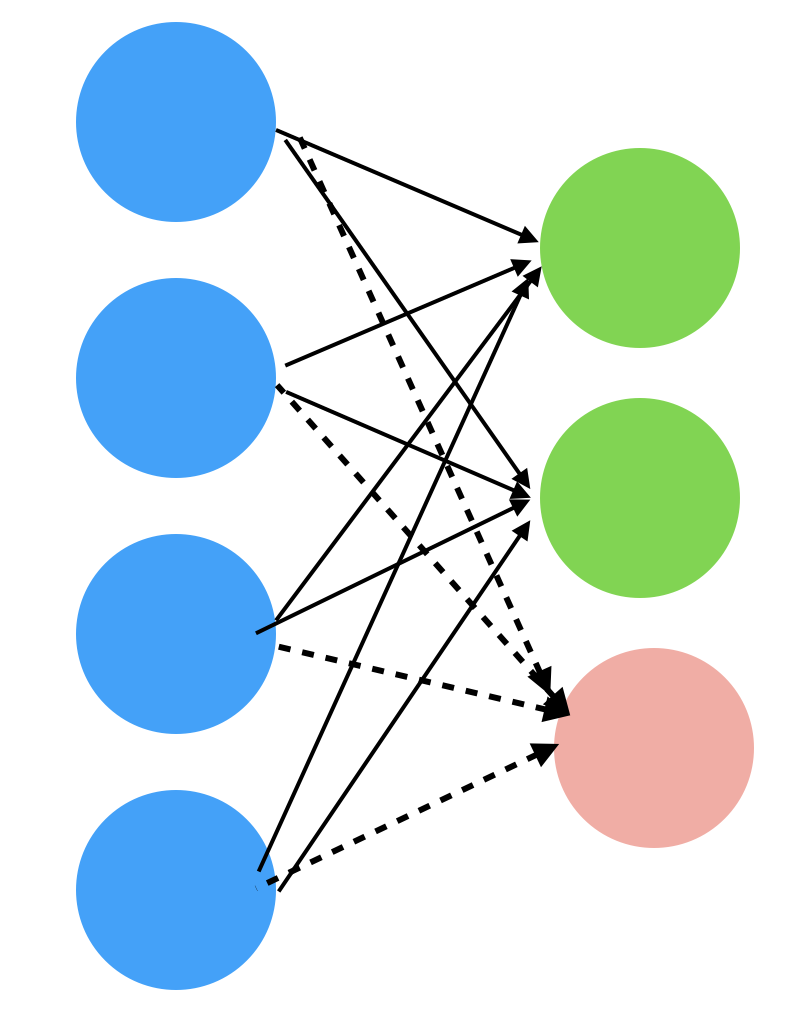
\includegraphics[width=8cm]{newclass.png}
	\bicaption[Illustration of the final linear layer tranformation for adding a new class]
	{增加类别时全连接层变化示意图}
	{Illustration of the final fully-connected layer tranformation for adding a new class. This figure assumes the case from 2 classes to 3 classes. The blue circles represent the feature map from the last layer. The green circles represent the class scores for the old two classes, and the red circle is the newly added class score output. The lines indicate weights, and dashed lines represent new weights to be added for the new class. A softmax layer follows this fully-connected layer.}
	\label{fig:newclass}
\end{figure}
The modifications to the output layer is illustrated in Fig.~\ref{fig:newclass}, and can be formalized as follows. The weights of the layers before the fully connected layer remains unchanged. This indicates that the output vector before the fully connected layer, i.e., the input vector to the fully connected layer is still denoted as $\mathbf{O}$, which is unchanged. Then the fully connected layer is modified as:
\begin{align}
f(\mathbf{O}; \hat{\mathbf{W_f}}, \hat{\mathbf{b_f}}) =  \hat{\mathbf{W_f}}\mathbf{O} + \hat{\mathbf{b_f}}
\end{align}
We construct the new weights and bias $\hat{\mathbf{W_f}}$ and $\hat{\mathbf{b_f}}$ as follows:
%这里可以放张示意图
\begin{align}
\left\{
	\begin{aligned}
	\hat{\mathbf{W_{f_{x,y}}}} & = & \mathbf{W_{f_{x,y}}}& ,& y = 1...N\\
	\hat{\mathbf{W_{f_{x,y}}}} & = & 0&,& y = N+1	
	\end{aligned}
\right.
\end{align}
\begin{align}
\left\{
\begin{aligned}
\hat{\mathbf{b_{f_{y}}}} & = & \mathbf{b_{f_{y}}}& ,& y = 1...N\\
\hat{\mathbf{b_{f_{y}}}} & = & 0&,& y = N+1	
\end{aligned}
\right.
\end{align}
We can also randomly initialize the added weights according to the neural networks' weight initialization convention, but the results differ little since they affect little on its gradients.

After this transformation, the output of the final fully connected layer $f(\mathbf{O}; \hat{\mathbf{W_f}}, \hat{\mathbf{b_f}})$ would be a $1\times (N+1)$ vector. After passing the vector to the softmax function, we are able to obtain class confidence scores for the $N+1$ classes. Let us denote the deep convolutional network after this transformation as $\Phi(x_i; \hat{\mathbf{W}})$, by substituting the parameters $\mathbf{W}$ with $\hat{\mathbf{W}}$.


\section{A Straightforward Method}

Utilizing the transformation method introduced in the previous section, we are ready to develop methods to train the newly added parameters, as well as continue training the trained parameters of the network. One baseline is to fix the old parameters and only train the newly added parameters in the final layer. However, this baseline algorithm performs so poorly that we do not mention in our experiments. Because the features are only trained on the first available classes, the network cannot learn better features later. We are going to discuss another baseline algorithm that makes more sense. Following the common practice of training deep neural networks, we will use Stochastic Gradient Descent\cite{he2016deep} (SGD) with momentum\cite{sutskever2013importance} as the default optimization algorithm to train the network. 

Let us first define the accuracy upper bound, which is the accuracy when the parameters $\mathbf{W}$ of deep convolutional network $\Phi(\mathbf{x_i}; \mathbf{W})$ is trained from scratch using the training set $\mathbb{X}\cup \hat{\mathbb{X}}$. It is clear that to obtain this upper bound, lots of training time would be needed. Since all data is used to train the network from scratch, the network will be able to learn more globally optimal and discriminative features to distinguish all $N+1$ class. The time and computation needed to obtain this accuracy upper bound would also be the upper bound of the cost of time and computation. Here, since more computation leads to longer time, we will use the terms computation and time interchangably. Because since it is impossible for other methods to improve the accuracy, the other methods with longer training time will have no meaning of existence compared to this method. The aim of our algorithm, would be to find methods that lie inside the computation upper bound, while maintaining a relatively high accuracy compared to the accuracy upper bound.

Considering this problem, a straightforward intuition is to use the training set data $\mathbb{X}$ as few as possible, since the current deep CNN can already classify the classes $1...N$. We can interpret this intuition as the knowledge of classifying classes $1...N$ is already captured by the current deep network $\Phi(\mathbf{x_i}; \mathbf{W})$. We hope the new network based on $\Phi(\mathbf{x_i}; \mathbf{W})$ can quickly learn additional knowledge to distinguish class $N+1$. 

Following the intuition, let us consider an extreme case. We will only use the new data, $\hat{\mathbb{X}}$ to further train the network $\Phi(x_i; \hat{\mathbf{W}})$. By only using the new data, we can save lots of computation, because on average the training set size would only be $\frac{1}{N+1}$ of the whole training set $\mathbb{X}\cup \hat{\mathbb{X}}$. Implementing this idea, the result is that the accuracy for the $N+1$ class will quickly rush to $100\%$, while the accuracy for classes $1...N$ will become $0$. This phenomenon can be explained in this way: Since the network can only see the class $N+1$, the loss would be completely biased towards the class $N+1$. Then, the gradients will quickly let the network output very high confidence on class $N+1$, and very low confidence on classes $1...N$. The gap between those confidence will become worse and worse as we train more and more epochs, because there is only training data for class $N+1$. Thus, we should discard this extreme method since it does not work at all.

However, the extreme case gives us some intuition to extend it to a better method. We can consider the other extreme, which is using the entire training set $\mathbb{X}\cup \hat{\mathbb{X}}$ to further train the network $\Phi(x_i; \hat{\mathbf{W}})$. Thus, it is obvious that we can extend these two extreme cases into a unified algorithm, using a hyper-parameter $\lambda$ to control the extent to which we use the old training set $\mathbb{X}$. The algorithm can be defined as in Algorithm \ref{algo:baseline}.


\begin{algorithm}
	\caption{A class-incremental learning baseline algorithm}
	\label{algo:baseline}
	\begin{algorithmic}
		\For{$i = 0 \to MAX\_EPOCH$} 
		\State \textbf{Step 1:} Randomly sample a subset $\mathbf{X}$ from the old training set $\mathbb{X}$, satisfying the size of the subset is $\lambda$ times the size of the old training set, i.e., $|\mathbf{X}| = \lambda|\mathbb{X}|$.
		\State \textbf{Step 2:} Use the combined training set $\mathbf{X} \cup \hat{\mathbb{X}}$ to train the network for an epoch using Stochastic Gradient Descent. By one epoch, we mean that each image $x_i \in \mathbf{X} \cup \hat{\mathbb{X}}$ is used and used exactly once to train the network.
		\State \textbf{Step 3:} Use the combined training set $\mathbf{X} \cup \hat{\mathbb{X}}$ to train the network for an epoch using our modified version of Stochastic Gradient Descent, following Equation \ref{sgdrule2}. By one epoch, we mean that each image $x_i \in \mathbf{X} \cup \hat{\mathbb{X}}$ is used and used exactly once to train the network.
		\EndFor
	\end{algorithmic}
\end{algorithm}

In our experiments, we found that this algorithm does not work well, because if $\lambda$ is not large enough, the outputs of the network will still be heavily biased to towards class $N+1$, similar to the extreme case described earlier. This is because the distribution of the number of different classes is different to the original distribution. On the other hand, if we used a large $\lambda$ to balance this issue, the computation cost will be too large since the entire old dataset $\mathbb{X}$ can be very large.

To cope with this issue, we further extended the algorithm, by adjusting the rules for Stochastic Gradient Descent. The general intuition is that, we hope to use a weighted loss instead of unweighted loss for different classes, so that the weights can balance the distribution to the original proportion of training image belonging to each class. For example, originally training data for class $N+1$ might only account for $\frac{1}{N+1}$ of the entire training set. Under our algorithm, it is possible that half of the temporary training set $\mathbf{X} \cup \hat{\mathbb{X}}$ belongs to class $N+1$. In this case, the network's outputs will be biased towards class $N+1$, giving more probability to class $N+1$. Then, we hope to give more weight to the loss of classes $1...N$, to adjust for this imbalance. Formally speaking, we can modify the Stochastic Gradient Descent with momentum rule to achieve this goal. The standard SGD with momentum update for one sample of data $x_i$ can be written as:
\begin{align}
\left\{
\begin{aligned}
	\upsilon_{t+1} &= m\upsilon_t + (1-m)\left( \eta g_i + \eta w_c \mathbf{W}_t \right)\\
	\mathbf{W}_{t+1} &= \mathbf{W}_{t} - \upsilon_{t+1}
\end{aligned}
\right.
\label{sgdrule}
\end{align}
where $\upsilon_t$ denotes the momentum at time step $t$, $\eta$ denote the hyper-parameter learning rate, $w_c$ denote the hyper-parameter weight decay, $m$ denote the hyper-parameter momentum coefficient, and $g_i$ denote the gradient for the data sample $x_i$, which is actually $g_i = \frac{\partial L_i}{\partial \mathbf{W}_t}$. Note that we normally train in batches of data instead of single examples to increase speed and stability. Then $g_i$ should be substituted with the average gradient of the batch of data. But we omit this detail here for simplicity.

We modify Equation \ref{sgdrule} into the following:
\begin{align}
\left\{
\begin{aligned}
\upsilon_{t+1} &= m\upsilon_t + (1-m)\left( \eta\beta\frac{1}{\lambda} g_i + \eta w_c \mathbf{W}_t \right)&, &   y_i \in \{1...N\}\\
\upsilon_{t+1} &= m\upsilon_t + (1-m)\left( \eta g_i + \eta w_c \mathbf{W}_t \right)&, &   y_i = N+1\\
\mathbf{W}_{t+1} &= \mathbf{W}_{t} - \upsilon_{t+1}
\end{aligned}
\right.
\label{sgdrule2}
\end{align}
where $y_i$ denote the ground truth label for the sample.

Shown in Equation \ref{sgdrule2}, we multiplied $g_i$ with two coefficients. The coefficient $\frac{1}{\lambda}$, comes from the sampled subset proportion factor $\lambda$, to re-weight the gradients, so that the proportion of every class are re-weighted to original proportion of the whole dataset. However, in our experiments, we found that simply re-weighting to the original proportion is not enough, perhaps because there is more noise coming from samples of classes $1...N$ because relatively fewer samples are used. Therefore, we introduced the hyper-parameter $\beta$, to further adjust the weights.

Let us analyze the computation needed in this baseline method, to better understand its speed. In every iteration, we train the deep neural network using $\lambda|\mathbb{X}| + |\hat{\mathbb{X}}|$ images. The computation needed divided by the computation of one entire epoch is formalized as Equation \ref{eq:baseline}. Because $|\hat{\mathbb{X}}|$ is very small compared to $|\mathbb{X}|$, we can omit it approximately.

\begin{align}
\frac{\lambda|\mathbb{X}| }{|\mathbb{X}| + |\hat{\mathbb{X}}|} \approx \lambda
\label{eq:baseline}
\end{align}

Thus, the computation of this algorithm in every iteration is nearly proportional to the value of $\lambda$.

This method seems quite straightforward, but has not been seen in any literature. Because its performance is not very satisfying, we will regard this method as a baseline method in the experiments. Our algorithm in this paper will be based on this baseline method, which will be introduced in the following section.
\label{baselinesection}

\section{Our proposed method}

Our intuition is to utilize hard negative mining techniques commonly used in object detection algorithms. Instead of randomly sampling from the old dataset, we prioritize the harder examples, so that we can minimize the data usage from the old dataset, thus saving significant training time. Depending on the actual inference and training speed ratio on hardware, we provide two algorithms for class incremental learning based on hard negative mining. The first case is when inference time is negligible compared to training time on the same set of images. The second case is when inference time and training time are comparable.

\subsection{Under Fast Inference Speed Condition}
Let us first consider a simpler case, where inference time can be neglected compared to training time. This case is impossible in real life currently, but we will explain why inference time can be much faster than training time and elaborate that this case is indeed possible in the future on specialized hardware.
\subsubsection{Model Inference Time analysis}
In an inference step for a batch of images, we will perform a forward on the deep neural network, and obtain the network's outputs to predict the classes to which the batch of images belong. A inference step typically include only one step:
\begin{enumerate}
	\item  Forward the network to calculate the outputs.
\end{enumerate}

In a training step for a batch, however, would be much more complicated. A training step typically consists of the following three parts:
\begin{enumerate}
	\item  Forward the network to calculate the outputs.
	\item Back-propagate the network to calculate the gradients of every parameter with regards to the loss.
	\item Update every parameter using an optimization algorithm like SGD with the gradients.
\end{enumerate}
Suppose there are $|\mathbf{W}|$ parameters in all in a convolutional network. Since the network is a directed acyclic graph (DAG), the forwarding and back-propagation time is similar since every node will be calculated once. Roughly speaking, without other optimizations, inference takes about $1/3$ of training time.

Moreover, the introduction of TensorRT toolkit by NVIDIA enabled even much faster inference speed. They used techniques like Precision Calibration, Layer and Tensor Fusion, Kernel Auto-Tuning, Dynamic Tensor Memory and Multi-Stream Execution, and enabled inference speed to be approximately $20\times$ faster on the same GPU.

\subsubsection{Algorithm}
Under such circumstances, we design our algorithm as the following steps in Algorithm \ref{algo:fast}. Note that $\lambda$ has the same meaning as in section \ref{baselinesection}.

\begin{algorithm}
\caption{Class-incremental learning based on Hard Mining under negligible inference time}
\label{algo:fast}
	\begin{algorithmic}
		\For{$i = 0 \to MAX\_EPOCH$} 
		\State \textbf{Step 1:} Do one round of inference on the old training set $\mathbb{X}$, and record the model's confidence score on the ground truth class. In the meantime, maintain a priority queue \textit{q} for every class, with a maximum total size of $\alpha \lambda |\mathbb{X}|$. The priority queue \textit{q} stores the $\alpha \lambda |\mathbb{X}|$ worst performing images. $\alpha$ is a hyper-parameter larger than $1$.
		\State \textbf{Step 2:} Randomly sample $\lambda|\mathbb{X}|$ images evenly from every class from the priority queue \textit{q}. We denote the sampled set of images as $\mathbf{X}$. 
		\State \textbf{Step 3:} Use the combined training set $\mathbf{X} \cup \hat{\mathbb{X}}$ to train the network for an epoch using our modified version of Stochastic Gradient Descent, following Equation \ref{sgdrule2}. By one epoch, we mean that each image $x_i \in \mathbf{X} \cup \hat{\mathbb{X}}$ is used and used exactly once to train the network.
		\EndFor
	\end{algorithmic}
\end{algorithm}

In Step 1, since inference is very fast, the time can be neglected. In Step 2 and Step 3, we train the deep neural network using $\lambda|\mathbb{X}| + |\hat{\mathbb{X}}|$ images. We can compare the data used in Step 2 and Step 3 to the entire dataset as
$\frac{\lambda|\mathbb{X}| + |\hat{\mathbb{X}}|}{|\mathbb{X}| + |\hat{\mathbb{X}}|}$. Therefore, in every iteration, the computation needed divided by the computation of one entire epoch is formalized as Equation \ref{eq:slow}.

\begin{align}
\frac{\lambda|\mathbb{X}| + |\hat{\mathbb{X}}|}{|\mathbb{X}| + |\hat{\mathbb{X}}|} \approx \lambda
\label{eq:slow}
\end{align}

Thus, the computation needed in this algorithm in every iteration is also nearly proportional to $\lambda$.

\subsection{Under Slow Inference Speed}

In many cases, we do not have such fast inference speed as illustrated in the previous section. For example, the toolkit TensorRT might degrade performance, and might not be available for all platforms. Moreover, we have to spend time optimizing the model's inference speed, before we can benefit from the fast inference speed. So usually, although inference speed is still much faster than training speed, the inference time spent on going through the whole training set is not bearable.

Under such case, we can no longer follow Step 1 in Algorithm \ref{algo:slow}, because it does not update the model at all, so the time cost would be too much. Alternatively, we can do a simple modification to Step 1. Instead of freezing the model and test on all old training data $\mathbb{X}$, we train the model on $\mathbb{X}\cup \hat{\mathbb{X}}$ in order not to waste time on testing. In this way, Step 1 is modified so that in this step the model gets trained, and in the mean time we collect the images that the model do not perform well in the priority queue \textit{q}. This modification actually involves an approximation. It is based on the assumption that the relative hardness of images does not change much as the model updates its parameter in the new version of Step 1. Fortunately, shown in the experiments, this modification does work well. The new algorithm can be summarized in Algorithm \ref{algo:slow}.

\begin{algorithm}
	\caption{Class-incremental learning based on Hard Mining for slow inference speed platforms}
	\label{algo:slow}
	\begin{algorithmic}
		\For{$i = 0 \to MAX\_EPOCH$} 
		\State \textbf{Step 1:} Do one round of training on the entire mixed training set $\mathbb{X}\cup \hat{\mathbb{X}}$, and record the model's confidence score on the ground truth class. In the meantime, maintain a priority queue \textit{q} for each class, with a maximum total size of $\alpha \lambda |\mathbb{X}|$. The priority queue \textit{q} stores the $\alpha \lambda |\mathbb{X}|$ worst performing images belonging to the old dataset $\mathbb{X}$.
		\State \textbf{Step 2:} Randomly sample $\lambda|\mathbb{X}|$ images evenly for every class from the priority queue \textit{q}. We denote the sampled set of images as $\mathbf{X}$. 
		\State \textbf{Step 3:} Use the combined training set $\mathbf{X} \cup \hat{\mathbb{X}}$ to train the network for an epoch using our modified version of Stochastic Gradient Descent, following Equation \ref{sgdrule2}.
		\EndFor
	\end{algorithmic}
\end{algorithm}

In Step 1, since we will train one epoch on the entire dataset, it takes the computation of training one epoch. In Step 2 and Step 3, we train the deep neural network using $\lambda|\mathbb{X}| + |\hat{\mathbb{X}}|$ images. As a comparison to the entire dataset, we can write the ratio as
$\frac{\lambda|\mathbb{X}| + |\hat{\mathbb{X}}|}{|\mathbb{X}| + |\hat{\mathbb{X}}|}$. To conclude, in every iteration, the computation needed divided by the computation of one entire epoch is formalized as Equation \ref{eq:slow}.

\begin{align}
\frac{(|\mathbb{X}| + |\hat{\mathbb{X}}|)+(\lambda|\mathbb{X}| + |\hat{\mathbb{X}}|)}{|\mathbb{X}| + |\hat{\mathbb{X}}|} \approx 1 + \lambda
\label{eq:slow}
\end{align}

Thus, the computation needed in this algorithm in every iteration is about training on $1+\lambda$ times of size to the entire training set size. By using low $\lambda$ such as $0.01$ in the experiments, the ratio can be near to 1. The drawback of this algorithm is also obvious: the ratio can never be greater than 1, so the speedup is limited. This means we will always have to train on every image of the entire training set for several times.




